\chapter{Application in VAHSS}
\label{ch:VAHSS}
In this chapter an application of the aggregated set membership proof will be presented and evaluated. As discussed in the introduction VAHSS constructions is one example of constructions where multiple data providers, henceforth denoted clients, participates. In this chapter a construction of VAHSS, where the verification is extended to also include the clients, will be presented. The verification of clients will be such that each clients has to prove that the shared secret is in an predetermined allowed set or range.
After having modified the VAHSS construction such that clients are verified, different methods for verifying clients will be compared. This will mainly focus on comparing the previously derived aggregated set membership proof presented in Construction \ref{alg:ZKSM-Agg} to the state of the art Bulletproofs. 



\section{Construction of VAHSS Using Homomorphic Hash Functions}
\label{sec:VAHSS-HSS}
%Consider $n$ clients and $m$ servers, to simplify notation define the two sets $\mathcal{N}=\{1,...,n\}$ and $\mathcal{M} = \{1,...,m\}$. Let $c_i$ and $x_i$ for $i\in\mathcal{N}$ denote the clients (data providers) and their respective data. Denote the servers by $s_j$, where $\:j\in\mathcal{M}$.
The construction of VAHSS that will be considered in this paper was originally presented in \cite{SumItUp}, and further implemented and benchmarked in \cite{VAHSS}. In \cite{SumItUp} three different constructions of VAHSS, was  introduced in this paper the construction that makes use of homomorphic hash functions for verification of servers will be considered.  

%In this section the construction of the Verifiable Additive Homomorphic Secret Sharing (VAHSS), that this paper aim to extend is presented. The goal is to extend the VAHSS such that it in addition to  the verification of servers computations client are also verified to be honest. This will be done  by verifying that they do not provide false data. Different methods for verifying the data provided by the clients is explained in the next section.

%Before extending the VAHSS construction to additionally verify clients and combining it with the aggregated set membership proof introduced in the previous chapters. The VAHSS construction considered will be explained briefly. 

It will be assumed that $n$ clients and $m$ servers participated in the VHASS construction. To simplify notation the two sets $\mathcal{N}=\{1,...,n\}$ and $\mathcal{M} = \{1,...,m\}$ are introduced. The clients are denoted $c_i$ for $i\in\mathcal{N}$ and their respective data $x_i$.  The servers in the construction will be refereed to $s_j$, $\:j\in\mathcal{M}$. Each client $c_i$, splits their secret, $x_i$, into $m$ shares, denoted $\{x_{ij}\}_{j\in\mathcal{M}}$. The clients then sends one share to each server. The servers receives shares from all $n$ clients and computes the partial sum $y_j = \sum_{i\in\mathcal{N}} x_{ij} $ and publishes the result. The final sum can then be computed by any party by summing the public partial sums, this gives $y = \sum_{j\in\mathcal{M}} y_j = \sum_{j\in\mathcal{M}} \sum_{i\in\mathcal{N}} x_{ij} = \sum_{i\in\mathcal{N}} \sum_{j\in\mathcal{M}} x_{ij} =   \sum_{i\in\mathcal{N}}x_i$.

%For AHSS constructions, the idea is that each client splits their secret, $x_i$, into $m$ shares, denoted $x_{ij}$. The clients then sends one share to each server. The servers receives shares from all $n$ clients and computes the partial sum $y_j = \sum_{i\in\mathcal{N}} x_{ij} $ and publishes the result. The final sum can then be computed by any party by summing the public partial sums, this gives $y = \sum_{j\in\mathcal{M}} y_j = \sum_{j\in\mathcal{M}} \sum_{i\in\mathcal{N}} x_{ij} =  \sum_{i\in\mathcal{N}}x_i$. For VHASS construction in addition to AHSS a proof $\sigma$ that verifies that the partial sums $y_j=  \sum_{i=1}^n  x_{ij} $,  for all $j\in\mathcal{M}$, is generated and published. This allows any party to verify the correctness of the servers computations.

The proof $\sigma$ of the servers computations is obtained accordingly.  Each client $c_i$, publishes a checksum $\tau_i= g^{x_i+R_i}$, where $x_i$ is the secret hidden by the distributed shares and $R_i\in_R\mathds{F}$ is such that $R_n=\phi(p) \lceil \frac{\sum_{i=1}^{n-1}R_i}{\phi(p)}\rceil - \sum_{i=1}^{n-1}R_i $. Each server $s_j$, computes a partial proof $\sigma_j = g^{y_j}$.  Finally the verification is done by checking if $\prod_{j\in\mathcal{M}} \sigma_j = \prod_{i\in\mathcal{N}}\tau_i\wedge \prod_{i\in\mathcal{N}}\tau_i = g^y$.  If this holds then the servers computations are proved to be done correctly. For a precise implementation and proof of correctness, security and verification the reader is refereed to the original paper, \cite{SumItUp}.
\begin{comment}
%\subsection*{Construction}
%The considered VAHSS, uses homomorphic hash functions to verify the servers computations, it was presented in \cite{SumItUp} and then implemented and evaluated in \cite{VAHSS}.

%The shares that hides the secrets are constructed by making use of a certain polynomial, $p_i$. For each client, $c_i$, let $\theta_{i1},...,\theta_{im}\in\mathds{F}\backslash\{0\}$ and $\lambda_{i1},...,\lambda_{im}\in\mathds{F}$ be chosen such that the following property for polynomial $p_i$ holds,
%\begin{align}
%\label{eq:pi(0)}
%p_i(0) = \sum_{j=1}^m \lambda_{ij}p_i(\theta_{ij}).
%\end{align}
%Then if  $c_i$ puts the shares to  $x_{ij}= \lambda_{ij}p_i(\theta_{ij})$, where  the polynomial $p_i(X)$ is a $t$-degree polynomial defined as $p_i(X) = x_i + \sum_{k=1}^t a_kX^k$. The sum of all shares is , $\sum_{j=1}^m x_{ij} = \sum_{j=1}^m \lambda_{ij}p_i(\theta_{ij})= p_i(0) = x_i$, thus the shares $x_{ij}$ adds up to the secret $x_i$  and the secret is perfectly hidden is not all shares used in the summation. 

%This idea is used in the VAHSS Construction \ref{alg:VAHSS-HSS}. The construction consists of the six PPT algorithms: \textbf{ShareSecret}, \textbf{PartialEval}, \textbf{PartialProof}, \textbf{FinalEval}, \textbf{FinalProof} and \textbf{Verify}. 

%The clients  executed the step \textbf{ShareSecret}, the servers \textbf{PartialEval} and \textbf{PartialProof} and the last three steps can be ran by anyone. A full description of the construction and all six algorithms is seen in Construction \ref{alg:VAHSS-HSS}.

%To obtain a secret sharing protocol, where any true subset of shares reviles no information about the secret they are origination from, the construction makes use the following polynomial. 
%For each client, $c_i$, let $\theta_{i1},...,\theta_{im}\in\mathds{F}\backslash\{0\}$ and $\lambda_{i1},...,\lambda_{im}\in\mathds{F}$ such that the following property for polynomial $p_i$ holds,
%\begin{align}
%\label{eq:pi(0)}
%p_i(0) = \sum_{j=1}^m \lambda_{ij}p_i(\theta_{ij}).
%\end{align}
%Note that is the step \textbf{ShareSecret} the shares are put to $x_{ij}= \lambda_{ij}p_i(\theta_{ij})$ and the polynomial $p_i(X)$ is a $t$-degree polynomial defined as $p_i(X) = x_i + \sum_{k=1}^t a_kX^k$, thus $\sum_{j=1}^m x_{ij} = \sum_{j=1}^m \lambda_{ij}p_i(\theta_{ij})= p_i(0) = x_i$, thus the shares $x_{ij}$ adds up to the secret $x_i$ if all shares are in the sum and the secret is hidden else. 


%To verify servers honesty a proof, denoted $\sigma$, relying on homomorphic secret sharing is constructed. Each server, $s_j$ publishes a partial proof $\sigma_j$, and it will then be possible for any party to verify the correctness of the aggregation. A detailed description is seen in Construction \ref{alg:VAHSS-HSS}.


%\begin{algorithm}
%\caption{\textbf{: Verifiable additive homomorphic secret sharing}}
%\label{alg:VAHSS-HSS}
%\textbf{Goal:} Construct and share the sum $\sum_{i=1}^n x_i$, where $x_i$ is a secret value known by client $c_i$, where $i\in\mathcal{N}$ without any client needing to revealing their individual secret. The servers, used to sharing the secrets, computations are verified so they must be honest. 
%\vspace{2pt}
%\hline 
%\vspace{2pt}
%\begin{itemize}
 % \item\textbf{ShareSecret $(1^\lambda,i,x_i)\xrightarrow[]{}(\tau_i,\{x_{ij}\}_{j\in\mathcal{M}})$}\\
%Pick uniformly at random $\{a_i\}_{i\in\{1,..,t\}}\in\mathds{F}$ and a $t$-degree polynomial $p_i$ on the form $p_i(X) = x_i + a_1X+...+a_tX^t$. Let $\mathcal{H}:x\mapsto g^x$
% (g generator the multiplicative group of $\mathds{F}$)
%, be a collision-resistant homomorphic hash function. Let $R_i\in\mathds{F}$ be the output of a PRF. Where it is required that  $R_n\in \mathds{F}$  satisfies
%$R_n = \phi(N)\lceil \frac{\sum_{i=1}^{n-1}R_i}{\phi(N)}\rceil- \sum_{i=1}^{n-1}R_i $. Compute $\tau_i = \mathcal{H}(x_i+R_i)$, and put $x_{ij}=\lambda_{i,j}p_i(\theta_{ij})$.  Output $\tau_i$ and $x_{i,j}$ for $j\in\mathcal{M}$. 

%\item\textbf{PartialEval $(j,\{x_{ij}\}_{i\in\mathcal{N}})\xrightarrow[]{}y_j$}\\
%Compute and output $y_j = \sum_{i=1}^n x_{ij}$.

%\item\textbf{PartialProof $(j,\{x_{ij}\}_{i\in\mathcal{N}})\xrightarrow[]{}\sigma_j$}\\
%Compute and output $\sigma_j = \prod_{i=1}^n g^{x_{ij}} =  g^{\sum_{i=1}^n x_{ij}}= g^{y_j}=\mathcal{H}(y_j)$.

%\item\textbf{FinalEval $(\{y_j\}_{j\in\mathcal{M}})\xrightarrow[]{}y$}\\
%Compute and output $y = \sum_{j=1}^m y_{j}$.

%\item\textbf{FinalProof $(\{\sigma_j\}_{j\in\mathcal{M}})\xrightarrow[]{}\sigma$}\\
%Compute and output $\sigma = \prod_{j=1}^m \sigma_j = \prod_{j=1}^m g^{y_{j}} =  g^{\sum_{j=1}^m y_{j}}= g^{y}=\mathcal{H}(y)$.

%\item\textbf{Verify $(\{\tau_i\}_{i\in\mathcal{N}},\sigma,y)\xrightarrow[]{}\{0,1\}$}\\
%Compute and output $\sigma= \prod_{i=1}^n \tau_i \wedge \prod_{i=1}^n \tau_i = \mathcal{H}(y)$.
%\end{itemize}
%\end{algorithm}

%\subsection*{Correctness, Security and Verifiability}
%A HSS and a AHSS construction should satisfy  two requirements: \textit{Correctness} and \textit{Security}. A VAHSS should also satisfy \textit{Verifiability}. The exact definition of the three requirements for Construction \ref{alg:VAHSS-HSS} is given in \cite{SumItUp} and Theorem \ref{thm:VAHSS_CSV} states that Construction \ref{alg:VAHSS-HSS} fulfils these requirements. 
%\begin{comment}
%\begin{itemize}
  %  \item \textbf{Correctness} It must hold that Pr$\Big[\textbf{Verify}(\{\tau_i\}_{i\in\mathcal{N}},\sigma,y)=1\Big]=1$. This means that with probability $1$ the output $y$ from \textbf{FinalEval} is accepted given all parties where honest and the protocol were executed correctly.
   % \item \textbf{Security} Let $T$ define the set of corrupted servers such that $|T|<m$, i.e at least one server is honest.  Denote a PPT adversary by $\mathcal{A}_1$ and let the Adv$(1^\lambda,\mathcal{A},T):= \text{Pr}[b' = b]-1/2$ be the advantage of $\mathcal{A}=\{\mathcal{A}_1,\mathcal{D}\}$ in guessing $b$ in the following experiment:
    %\begin{enumerate}
      %  \item The adversary $\mathcal{A}_1$ gives $(i,x_i,x_i')$ to the challenger, where $i\in[n], x_i\neq x_i'$ and $|x_i|=|x_i'|$.
     %   \item The challenger picks a bit $b\in\{0,1\}$ uniformly at random chooses and computes $\textbf{ShareSecret}(1^\lambda,i,\hat{x}_i) = (\hat{\text{share}}_{i1},...,\hat{\text{share}}_{im},\tau_i)$, where $\hat{\textbf{x}}_i$ is  such that $\hat{x}_i = \begin{cases}x_i, \text{ if } b=0 \\ x_i' \text{ else} \end{cases}$. 
       % \item Given the shares from the corrupted servers T and $\hat{\tau}_i$ the adversary distinguisger outputs a guess $b'\xleftarrow[]{}\mathcal{D}((\hat{\text{share}_{ij}})_{j|s_j\in T},\hat{\tau}_i)$.
    %\end{enumerate}
    %A VAHSS-construction is $t$-secure if for all $T\subset \{s_1,...,s_m\}$ with $|T|<t$ it holds that Adv$(1^\lambda,\mathcal{A},T)<\varepsilon(\lambda)$ for some negligible $\varepsilon(\lambda)$.
 %\item \textbf{Verifiability} Let $\mathcal{A}$ denote any PPT  adversary and $T$ denote the set of corrupted servers with $T\leq m$. The verifiability property requires that any $\mathcal{A}$ who can modify the input shares to all servers $s_j\in T$ can cause a wrong value to be excepted as $y=f(x_1,...,x_n)$ with negligible probability.   
%\end{itemize}
%The VHASS in Construction \ref{alg:VAHSS-HSS} satisfies the correctness, security and verifiability requirements defined above, this is stated in Theorem \ref{thm:VAHSS_CSV} .
%\end{comment}

%\begin{thm}
%\label{thm:VAHSS_CSV}
%Construction \ref{alg:VAHSS-HSS} satisfies the correctness, security and verifiability requirements defined in \cite{SumItUp}.
%\end{thm}
%\begin{proof}
%See section $4.1$ in \cite{SumItUp}.
%\end{proof}
\end{comment}

\section{Additive homomorphic secret sharing with verification of both clients and servers }
\label{sec:combination}

The VAHSS construction discussed in section \ref{sec:VAHSS-HSS} assumes honest clients and verifiers the servers. The aim of this section is to extended the VAHSS construction to verify both clients and servers, without the clients needing to reveal their secrets. This will achieved by first deriving a client and server VAHSS, where the clients are verified using range proofs or set membership proofs based on a Pedersen commitment. Then it will also be discussed how such an construction would need to be modified to use instead aggregates set membership proofs. 

Remark that if a range proof or set membership proof is included in the VAHSS construction then potentially malicious clients can only have a limited influence on the computed sum. Range proofs and set membership proofs forces malicious input to still be part of the range or set. This leads to that the impact on the sum that a malicious client can have is bounded by the size of the range or the elements in the set. 

\subsection*{Client and Server VAHSS}
In this section it will be investigated how to combine the VHASS construction with a range proofs or set membership proofs.  Only range proofs and set membership proofs emanate from a Pedersen commitment hiding a secret and generates a zero knowledge proof that this secret belongs to an pre-specified interval or set will be considered. 

Note that to ensure honest clients it is not sufficient to construct and perform a set membership proof and VAHSS scheme separately. In such a protocol the verifier cannot be sure that the secret proven to be in the allowed set is the same as the secret hidden by the shares. The same holds considering range proofs.

Using the Pedersen commitment to link the VAHSS construction with a range proof or set membership proof, would result in a general construction of a client and server VAHSS compatible with any range proof or set membership proof enumerating from a Pedersen commitment. To obtain such a general construction of a client and server VAHSS the Pedersen commitment will be investigated if it can be implemented in the VAHSS construction. 

A connection between the shares generated in the algorithm \textbf{ShareSecret} in the VAHSS construction and the secret hidden in an Pedersen commitment is desired. Proving that the sum of the shares is equal to the secret in an Pedersen commitment and then providing a zero knowledge range proof or set membership proof for the commitment, would convince the verifier that the shares represents a secrets that is in the allowed range.  

Publishing a Pedersen commitment of the secret itself does not provide any guarantee that it is the same secret that is hidden by the shares. It can also be seen that committing to the shares in Pedersen commitments does not ensure the verifier that the secret hidden in the shares are in the allowed set or range. This is since the individual shares themselves does not reveal information about the secret they are hiding. This leads to that there is not guarantee that proving a share belongs to the allowed range (or set) implies that the secret does and the other way assuming that the secret to a range (or set) does not imply that the shares does.

%Thus some trick to connect the secret in the shares to the secret in the Pedersen commitment must be derived. Therefore  that the aggregation of the partial proofs used in the VAHSS construction to prove the honesty of the servers will be used to connect the range proofs to the VAHSS construction.

Recall that the clients in addition to the shares also publishes the checksum $\tau_i$ for the secret $x_i$, further recall that the definition of the checksum is  $\tau_i=g^{x_i+R_i}$, where $R_i$ is chosen uniformly at random from the field $\mathds{F}$ such that $R_n =\phi(p) \lceil \frac{\sum_{i=1}^{n-1}R_i}{\phi(p)}\rceil - \sum_{i=1}^{n-1}R_i$. 

The checksum $\tau_i$ can be seen as a generalisation of a Pedersen commitment. Therefore the  checksum may be used as a Pedersen commitment in the construction of a range proof  or set membership proof. Formally the checksum is a Pedersen commitment where $g=h$. However if $g=h$ the computationally binding property of a Pedersen commitment would not hold since $log_g(h)=log_g(g)=1$ which leads to that the left hand side in equation \eqref{eq:pedersen_binidng} is equal to $1$. Therefore to construct two commits $\mathds{E}(x,R)$ and $\mathds{E}(x',R')$ such that $\mathds{E}(x,R) = \mathds{E}(x',R')$ but $x\neq x'$ it is sufficient to solve solve for $x'$ in, 
\begin{align*}
R'-R = x-x'\:mod \:p .
\end{align*}
In other words it is straightforward to create a false commitment hence also a false range proof and set membership proof.

Instead investigated if the checksum $\tau_i$ can be modified into a Pedersen commitment where $g\neq h$. This leads to that instead of the previously computed checksum $\tau_i$,  the clients compute and output $\pi_i=g^{x_i}h^{R_i}$ , where $x_i,R_i,g,h$ are as above.

Given the commitment $\pi_i$ the clients can use it to construct a range proof or set membership proof of the secret in the commitment.  It remains to argue that this method ensures the verifier that the secret hidden by the shares is the same secret as in the commitment $\pi_i$ for $i\in\mathcal{N}$ that are used to prove honest clients.

Assume that client $c_k$ commits to the value $\hat{x}_k$ in the Pedersen commitment $\pi_k$ and constructs shares, $x_k_j$ such that $x_k = \sum_{j\in\mathcal{M}}x_{kj} \neq \hat{x}_k$. This leads to that $c_k$ generates a range proof that the secret hidden in the commitment belongs to the interval $[a,b]$ but the secret hidden by the shares does not necessarily belong to the range or set. Then the verification of the servers will not hold, since  $\prod_{i=1}^m \pi_i \neq g^y$. this means that the verification will return false and the protocol will not succeed, even if all  range proofs verifies true. Thus any cheating party will be detected, it will not be possible do determine which party that cheated and more precisely not even if the cheating party was a client or a server. 

In Construction \ref{alg:VAHSS-HSS-RP} the extended VAHSS, such that the construction ensures honest clients by including a range proof or set membership proof is described in detail. In order to clarify the modifications made to include a verification of the clients, the differences to the VAHSS construction presented in \cite{SumItUp} are pointed out. The algorithms \textbf{ShareSecret} and \textbf{Verify} has been modified,  and the algorithms \textbf{RangeProof} and \textbf{GenerateCommitment} have been added. More precisely in the algorithm \textbf{ShareSecret} does not output the checksum $\tau_i$, instead the Pedersen commitment $\pi_i$ is computed in the algorithm \textbf{GenerateCommitment}. The algorithm  \textbf{GenerateCommitment} can be included in either \textbf{ShareSecret}  or \textbf{RangeProof} instead of being viewed as a separate algorithm. In the implementation discussed later the commitment is generated while constructing the range proof and not explicitly. The algorithm \textbf{RangeProof} constructs a range proof (or set membership proof) denoted $\Sigma_i$ given the commitment $\pi_i$. It is not specified which range proof or set membership proof that is used to verify clients.  Which range proof or set membership proof that is used does not affect the rest of Construction \ref{alg:VAHSS-HSS-RP}, as long as it emanate from a Pedersen commitment, hence it is left unspecified. In addition to the steps in the algorithm \textbf{Verify} for the VAHSS presented in \cite{SumItUp}, the algorithm \textbf{Verify} verifies the correctness of the proofs $\Sigma_i$ and an additional \texttt{AND} operator to compute the total verification.  

The algorithms \textbf{GenereateCommitment} and \textbf{RangeProof} are executed by the clients and the other algorithms are executed by the same party as in the  VAHSS construction in \cite{SumItUp}. 

%In the VAHSS Construction \ref{alg:VAHSS-HSS} the verifiability property includes verification of the servers. In this section this will be extended to also include the clients. The value $\pi_i$ published by the clients will be modified into a Pedersen commitment on the form $\pi_i = g^{x_i}h^{R_i}$, remember $\pi_i=g^{x_i+R_i}$ in the original construction presented in \cite{SumItUp}. The clients will apart from the previous commitments  also construct and publish a range proof for $\pi_i$. This allows any verifier to apart from verifying the servers also verify that the secret shared by the clients is in an certain range.  

%Given this construction the correctness, security and verification requirements for the server verifiable AHSS presented in \cite{SumItUp} is still fulfilled  that should be fulfilled is redefined below.  The difference to the requirements for the server verifiable AHSS is that additional demands for the clients behaviour is included. 

\begin{comment}
\begin{itemize}
    \item \textbf{Correctness} It must hold that Pr$\Big[\textbf{Verify}(\{\pi_i\}_{i\in\mathcal{N}},\sigma,y,\{\Sigma_i\}_{i\in\mathcal{N}})=1\Big]=1$. This means that with probability $1$ the output $y$ from \textbf{FinalEval} is accepted given all parties (clients and servers) where honest and the protocol were executed correctly.
    \item \textbf{Security} 
    			\begin{itemize}
    						\item \textbf{Malicious Servers } The construction should satisfy the same security argument as the VAHSS-HSS construction in \cite{SumItUp}.
    						%Let $T$ define the set of corrupted servers such that $|T|<m$, i.e at 					least one server is honest.  										Denote a PPT adversary by $\mathcal{A}_1$ and let the Adv$(1^			\lambda,\mathcal{A},T):= \text{Pr}[b' = b]-1/2$ be the advantage 										of $\mathcal{A}=\{\mathcal{A}_1,\mathcal{D}\}$ in guessing $b$ in the following experiment:
    							%		\begin{enumerate}
       						%				 \item The adversary $\mathcal{A}_1$ gives $(i,x_i,x_i')$ to the challenger, where $i\in[n], x_i\neq x_i'$ and $|x_i|=|x_i'|$.
        						%				\item The challenger picks a bit $b\in\{0,1\}$ uniformly at random chooses and computes $\textbf{ShareSecret}(1^\lambda,i,																\hat{x}_i) = (\hat{\text{share}}_{i1},...,\hat{\text{share}}_{im},\tau_i)$, where $\hat{\textbf{x}}_i$ is  such that $\hat{x}_i = 																\begin{cases}x_i, \text{ if } b=0 \\ x_i' \text{ else} \end{cases}$. 
        					%					\item Given the shares from the corrupted servers T and $\hat{\tau}_i$ the adversary distinguisger outputs a guess 																			$b'\xleftarrow[]{}\mathcal{D}((\hat{\text{share}_{ij}})_{j|s_j\in T},\hat{\tau}_i)$.
   									% \end{enumerate}
    							%		A VAHSS-construction is $t$-secure if for all $T\subset \{s_1,...,s_m\}$ with $|T|<t$ it holds that Adv$(1^\lambda,\mathcal{A},T)<												\varepsilon(\lambda)$ for some negligible $\varepsilon(\lambda)$.
  					  \item \textbf{Malicious Clients}  Since the construction does not clarify the exact range proof used, the security argument is refereed to the original papers for the used range proof and by proving that the secret hidden by the Pedersen commitments is the same as the secrets in the shares. 
   		 \end{itemize} 
 	\item \textbf{Verifiability} 
 			\begin{itemize}
 						\item \textbf{Verify Servers }Let $\mathcal{A}$ denote any PPT  adversary and $T$ denote the set of corrupted servers with $T\leq m$. The verifiability 							property requires that any $\mathcal{A}$ who can modify the input shares to all servers $s_j\in T$ can cause a wrong value to be excepted as 							$y=f(x_1,...,x_n)$ with negligible probability.   
 						\item \textbf{Verify Clients} Let $\mathcal{A}$ denote any PPT adversary and $T$ denote the set of corrupted clients. The verifiability property requires that any $\mathcal{A}$ who can modify the Pedersen commitments $\pi_i$  to any $\pi_i^{'} \:\forall  i\in T$ has a negligible probability at choosing a commitment $\pi_i^{'}$ such that Verify$( \{\pi^{'}_i\}_{i\in\mathcal{N}},x,y)=1$.
 			\end{itemize} 
\end{itemize}
\end{comment}

\begin{algorithm}
\caption{\textbf{: Client and Server Verifiable additive homomorphic secret sharing}}

\textbf{Goal:} Construct and share the sum $\sum_{i=1}^n x_i$, where $x_i$ is a secret value known by client $c_i$, where $i\in\mathcal{N}$ without any client needing to revealing their individual secret. All parties are verified to be honest in the construction.
\vspace{2pt}
\hline
\vspace{2pt}
\begin{itemize}
 \item\textbf{ShareSecret $(1^\lambda,i,x_i) \mapsto \{x_{ij}\}_{j\in\mathcal{M}}$} \\
Pick uniformly at random $\{a_i\}_{i\in\{1,..,t\}}\in_R\mathds{F}$ to be the coefficients to a $t$-degree polynomial $p_i$ on the form $p_i(X) = x_i + a_1X+...+a_tX^t$. Define  the shares as $x_{ij}=\lambda_{i,j}p_i(\theta_{ij})$ for $j\in\mathcal{M}$, the parameters $\theta_{ij}$ and Lagrange coefficients $\lambda_{ij}$ is chosen such that equation \ref{eq:pi(0)} is satisfied.
Output $\{x_{ij}\}_{j\in\mathcal{M}}$.

\item\textbf{GenereteCommitment$(1^\lambda,i,x_i) \mapsto \pi_i$ }\\
Let $\mathds{E} : x,y \to g^xh^y$ be a Pedersen commitment . Let $R_i\in\mathds{F}$ be the output of a PRF such that $R_n\in \mathds{F}$  satisfies $R_n = \phi(N)\lceil \frac{\sum_{i=1}^{n-1}R_i}{\phi(N)}\rceil- \sum_{i=1}^{n-1}R_i $. Compute and output $\pi_i = \mathds{E}(x_i,R_i)$.

\item\textbf{RangeProof $(pp,x_i,\pi_i) \mapsto \Sigma_i$}\\
Construct a range proof or set membership proof, denoted $\Sigma_i$, for the Pedersen commitment $\pi_i$ of the secret $x_i$, on the  range $[0,B]$ or a set $\Phi$. All required public parameters, $pp$, needed to  construction the proof $\Sigma_i$ is assumed to be pre-shared and known by all parties.
\item\textbf{PartialEval $(j,\{x_{ij}\}_{i\in\mathcal{N}})\xrightarrow[]{}y_j$}\\
Compute and output $y_j = \sum_{i=1}^n x_{ij}$.

\item\textbf{PartialProof $(j,\{x_{ij}\}_{i\in\mathcal{N}})\xrightarrow[]{}\sigma_j$}\\
Compute and output $\sigma_j = \prod_{i=1}^n g^{x_{ij}} =  g^{\sum_{i=1}^n x_{ij}}= g^{y_j}=H(y_j)$.

\item\textbf{FinalEval $(\{y_j\}_{j\in\mathcal{M}})\xrightarrow[]{}y$}\\
Compute and output $y = \sum_{j=1}^m y_{j}$.

\item\textbf{FinalProof $(\{\sigma_j\}_{j\in\mathcal{M}})\xrightarrow[]{}\sigma$}\\
Compute and output $\sigma = \prod_{j=1}^m \sigma_j = \prod_{j=1}^m g^{y_{j}} =  g^{\sum_{j=1}^m y_{j}}= g^{y}=H(y)$.

\item\textbf{Verify $(\{\pi_i\}_{i\in\mathcal{N}},x,y,\{\Sigma_i\}_{i\in\mathcal{N}})\xrightarrow[]{}\{0,1\}$}\\
Compute and output $\sigma= \prod_{i=1}^n \pi_i \wedge \prod_{i=1}^n \pi_i = H(y)\wedge \{\textbf{VerifyClients}( \Sigma_i) \}_{i\in\mathcal{N}}$. Where $\textbf{VerifyClients}$ is the verification algorithm associated with the algorithm used by the clients to construct the proofs $\{\Sigma_i\}_{i\in\mathcal{N}}$.
\end{itemize}
\label{alg:VAHSS-HSS-RP}
\end{algorithm}

\begin{thm}
\label{thm:VAHSS_RP_CSV}
\vspace{10pt}
The client and server VAHSS presented in Construction \ref{alg:VAHSS-HSS-RP} satisfies the correctness, security and verifiability requirements described in section \ref{sec:VAHSS-HSS}, by replacing $\tau_i$ with $\pi_i$. Additionally it also satisfies the following extension of the verification requirement:

Let $\mathcal{A}$ denote any PPT adversary and $T$ denote the set of corrupted clients. The extended verifiability property requires that any $\mathcal{A}$ who can modify the Pedersen commitments $\pi_i$  to any $\pi_i^{'} \:\forall  i\in T$ has a negligible probability at choosing a commitment $\pi_i^{'}$ such that Verify$( \{\pi^{'}_i\}_{i\in\mathcal{N}},x,y,\{\Sigma_i\}_{i\in\mathcal{N}})=1$.



%\begin{itemize}
 %\item \textbf{Verifiability Servers}  Let $\mathcal{A}$ denote any PPT  adversary and $T$ denote the set of corrupted servers with $T\leq m$. Note that if $|T|=m$, the verifiability property holds but not the security property. The verifiability property requires that any $\mathcal{A}$ who can modify the input shares to all servers $s_j\in T$ can cause a wrong value to be excepted as $y=f(x_1,...,x_n)$ with negligible probability.  
 %\item  \textbf{Verifiability Clients} 
%\end{itemize} 

\end{thm}
%TODO fix proof before hand in to Seminar 2
\begin{proof}
To argue that that the correctness, security and verifiability properties for the VAHSS still holds after replacing  $\tau_i$ with $\pi_i$ for $i=1,...,n$, it is noted that,
\begin{align*}
&\prod_{i=1}^n \pi_i = \prod_{i=1}^n g^{x_i}h^{R_i} = g^{\sum_{i=1}^n x_i}h^{\sum_{i=1}^n R_i} = g^{\sum_{i=1}^n} h^{ \phi(N)\big\lceil \frac{\sum_{i=1}^{n-1}R_i}{\phi(N) }\big\rceil} = g^y \\
&\text{Hence it follows that: } \prod_{i=1}^n \tau_i = \prod_{i=1}^n \pi_i.
\end{align*}
Further the Pedersen commitment is perfectly hiding and computationally binding and hence it follows that the requirements is still fulfilled. 

It remains to prove that Construction \ref{alg:VAHSS-HSS-RP} also fulfils the extended verification requirement. This follows from the soundness of the range proofs or set membership proof used in the construction and by the argument above that the secret hidden in the commitment $\pi_i$ must be the same as the secret obtain by combining the the shares $\{x_{ij}\}_{j\in\mathcal{M}}$ for all $i=1,...,n$.

\begin{comment}
The correctness follows from the correctness of range proofs and by proving that $\sigma= \prod_{i=1}^n \pi_i \:\bigwedge\: \prod_{i=1}^n \pi_i = \mathcal{H}(y)$. Both $y$ and $\sigma$ are the same as in Construction \ref{alg:VAHSS-HSS}, hence by construction:
\begin{align}
    \label{eq:y=sum(x_ij)}
    y = \sum_{j=1}^m y_j= \sum_{j=1}^m \sum_{i=1}^n \lambda_{ij}p_i(\theta_{ij}) = \sum_{i=1}^n \overbrace{ \Big (\sum_{j=1}^m \lambda_{ij}p_i(\theta_{ij}) \Big)}^{ p_i(0)} = \sum_{i=1}^n p_i(0) = \sum_{i=1}^n x_i,
\end{align}
and for $\sigma$ it holds that:
\begin{align*}
    \sigma = \prod_{j=1}^m \sigma_j = \prod_{j=1}^m g^{y_j} = g^{\sum_{j=1}^my_j} =g^y = \mathcal{H}(y)
\end{align*}
For the $\pi_i$, whose construction has been modified compared to $\tau_i$ in  Construction\ref{alg:VAHSS-HSS}, thus it follows that:
\begin{align*}
    &\prod_{i=1}^n \pi_i = \prod_{i=1}^n \mathds{E}(x_i,R_i)= \prod_{i=1}^n g^{x_i}h^{R_i} = g^{\sum_{i=1}^n x_i } h^{\sum_{i=1}^n R_i} \overset{\eqref{eq:y=sum(x_ij)}}{=} g^y h^{\sum_{i=1}^{n-1} R_i+R_n} = \\ 
    &= g^y h^{ \phi(N)\big\lceil \frac{\sum_{i=1}^{n-1}R_i}{\phi(N) }\big\rceil} = g^y = \mathcal{H}(y) 
\end{align*}

The proof of security argument for malicious servers given in \cite{SumItUp} is still sufficient since the Pedersen commitment is perfectly hiding and computationally binding and that the range proofs are zero knowledge. The security argument for malicious clients follows from the soundness of the range proof and that the secret hidden in the commitment has to be the same as the secret in the shares, as argued above. . 

The proof of \textit{\textbf{Verifiability Severs}} is the same as the proof given in  in \cite{SumItUp}, except that the commitments $\pi_i$ replaces the checksums $\tau_i$.  \textit{\textbf{Verifiability Clients}} follows from the properties of the range proof.
\end{comment}
\end{proof}

\subsection*{Combining with aggregated set membership proof}
When using the aggregated set membership to verify the clients in a VHASS construction Theorem \ref{thm:aggrgeation} do not hold if the aggregation is performed by one untrusted server, since the assumptions are not fulfilled.  The sum of secrets can be computed by any party after all servers has performed the algorithm \textbf{partialEval} and it is known that $h^{\sum_{i\in\mathcal{N}} R_i } =1 \: \text{mod}\:  \phi(p)$. Thereby although the individual secrets are unknown, it is possible to cheat by using the fact that $y=\sum_{i\in\mathcal{N}}x_i, h^{\sum_{i\in\mathcal{N}}R_i}$ are known. To illustrate how this information can be use to cheat consider, $D=C^{k+c}, z_R = k\phi (N)$ and $z_x = k y$, where $y= \sum_{i=1}^n x_i$ and $k\in_R \mathds{F}$, it follows that, 
\begin{align*}
LHS =& D = C^{k+c}= \big( g^ { k \sum_{i=1}^n x_i } h^{ k  \sum_{i=1}^n R_i ) } \big)   \big( g^{ (  \prod_{i=1}^n c_i ) \sum_{i=1}^n x_i ) } h^{ ( \prod_{i=1}^n c_i ) \sum_{i=1}^n R_i ) } \big)   \\
LHS =& C^c h^{z_R}g^{z_x} = C^c h^{k \phi (N) } g^{k y} =  \big( g^{ (  \prod_{i=1}^n c_i ) \sum_{i=1}^n x_i ) } h^{ ( \prod_{i=1}^n c_i ) \sum_{i=1}^n R_i ) } \big) h^{k\phi (N)} g^{ky}\\
= &  \big( g^{ (  \prod_{i=1}^n c_i ) \sum_{i=1}^n x_i ) } h^{ ( \prod_{i=1}^n c_i ) \sum_{i=1}^n R_i ) } \big)g^ { k y} h^{ k  \phi(N)\lceil \frac{\sum_{i=1}^{n-1}R_i}{\phi(N)}\rceil ) }\\
& \implies LHS= RHS.
\end{align*}
Thus it follows that Theorem \ref{thm:aggrgeation} does not hold when one untrusted part aggregates all clients set membership proofs in a client and server VHASS. 
%Further it is seen that  it is possible for such an aggregating party to  cheat and provide an aggregated proof that  verifies true without the statement in equation \eqref{eq:SM_statement} being true.

If instead of one party that aggregates all set membership proofs, if multiple parties aggregates subsets of the proofs, Theorem \ref{thm:aggrgeation} would hold. This follows from the fact that the sum of the secrets and random values would be unknown to the aggregating party. The construction of the aggregated client and server VAHSS construction for untrusted aggregating parties is presented in Construction \ref{alg:VAHSS-HSS-RP-Agg}.



\begin{algorithm}
\caption{\textbf{: Client and Server Verifiable additive homomorphic secret sharing}}

\textbf{Goal:} Construct and share the sum $\sum_{i=1}^n x_i$, where $x_i$ is a secret value known by client $c_i$, where $i\in\mathcal{N}$ without any client needing to revealing their individual secret. All parties are verified to be honest in the construction.
\vspace{2pt}
\hline
\vspace{2pt}
\begin{itemize}
 \item\textbf{ShareSecret $(1^\lambda,i,x_i) \mapsto \{x_{ij}\}_{j\in\mathcal{M}}$} \\
Pick uniformly at random $\{a_i\}_{i\in\{1,..,t\}}\in_R\mathds{F}$ to be the coefficients to a $t$-degree polynomial $p_i$ on the form $p_i(X) = x_i + a_1X+...+a_tX^t$. Define  the shares as $x_{ij}=\lambda_{i,j}p_i(\theta_{ij})$ for $j\in\mathcal{M}$, the parameters $\theta_{ij}$ and Lagrange coefficients $\lambda_{ij}$ is chosen such that equation \ref{eq:pi(0)} is satisfied.
Output $\{x_{ij}\}_{j\in\mathcal{M}}$.

\item\textbf{GenereteCommitment$(1^\lambda,i,x_i) \mapsto \pi_i$ }\\
Let $\mathds{E} : x,y \to g^xh^y$ be a Pedersen commitment . Let $R_i\in\mathds{F}$ be the output of a PRF such that $R_n\in \mathds{F}$  satisfies $R_n = \phi(N)\lceil \frac{\sum_{i=1}^{n-1}R_i}{\phi(N)}\rceil- \sum_{i=1}^{n-1}R_i $. Compute and output $\pi_i = \mathds{E}(x_i,R_i)$.

\item\textbf{RangeProof $(pp,x_i,\pi_i) \mapsto \Sigma_i$}\\
Construct a range proof, denoted $\Sigma_i$, for the commitment $\pi_i$ to the secret $x_i$, on the set $\Phi$ using the algorithm \textbf{Prove} in Construction \ref{alg:ZKSM-Agg}. All required pubic parameters a $pp$ is assumed to be pre-shared and known by all parties.

\item\textbf{PartialEval $(j,\{x_{ij}\}_{i\in\mathcal{N}})\xrightarrow[]{}y_j$}\\
Compute and output $y_j = \sum_{i=1}^n x_{ij}$.

\item\textbf{PartialProof $(j,\{x_{ij}\}_{i\in\mathcal{N}})\xrightarrow[]{}\sigma_j$}\\
Compute and output $\sigma_j = \prod_{i=1}^n g^{x_{ij}} =  g^{\sum_{i=1}^n x_{ij}}= g^{y_j}=H(y_j)$.

\item \text{\textbf{PartialAggregate} $(pp,k,\mathcal{S}_k, \{\Sigma_i\}_{i\in\mathcal{S}} ) \xrightarrow[]{} \Sigma_{a_k}}$} \\
Given a subset of proofs  $\{ \Sigma_i}\}_{i\in\mathcal{S}_k}$ where $\mathcal{S}_k\subseteq\{1,...,n\}$. Aggregate the set of proof according to the algorithm \textbf{Aggregate} in Construction \ref{alg:ZKSM-Agg}. Publish the aggregates proof $\Sigma_{a_k}$. 


\item\textbf{FinalEval $(\{y_j\}_{j\in\mathcal{M}})\xrightarrow[]{}y$}\\
Compute and output $y = \sum_{j=1}^m y_{j}$.

\item\textbf{FinalProof $(\{\sigma_j\}_{j\in\mathcal{M}})\xrightarrow[]{}\sigma$}\\
Compute and output $\sigma = \prod_{j=1}^m \sigma_j = \prod_{j=1}^m g^{y_{j}} =  g^{\sum_{j=1}^m y_{j}}= g^{y}=H(y)$.

\item\textbf{Verify $(\{\pi_i\}_{i\in\mathcal{N}},x,y,\{\Sigma_{a_k}}\}_{j\in\mathcal{K}})\xrightarrow[]{}\{0,1\}$}\\
Compute and output $\sigma= \prod_{i=1}^n \pi_i \wedge \prod_{i=1}^n \pi_i = H(y)\wedge \{\textbf{VerifyClients}(\Sigma_{a_k})\}_{k\in\mathcal{K}}$. Where $\textbf{VerifyClients}$ is the verification algorithm in Construction \ref{alg:ZKSM-Agg}.
\end{itemize}
\label{alg:VAHSS-HSS-RP-Agg}
\end{algorithm}


%If the sum of $\sum_{i=1}^n x_i$ and $\sum_{i=1}^nR_i$ where unknown then the aggregation party would have to choose the values $z_x$ and $z_R$ such that,
%\begin{align*}
%h^{z_R}g^{z_x} \overset{!}{=} g^{k\sum_{i=1}^n x_i }h^{k\sum_{i=1}^n R_i } = \Big( g^{k\sum_{i=1}^n R_i}h^{k\sum_{i=1}^n R_i}\Big)^k,
%\end{align*}
%which is the same as construction two equal Pedersen commitments, which is assumed to be impossible due to that the $log_g h$ is unknown. 

For the VAHSS construction this can be implemented by letting the server, which computes the partial sums, aggregate different subset of the clients set membership proofs. For example in the case of $100$ clients and $5$ servers, each server aggregates $20$ proofs. For example this could be implemented by $\mathcal{K} = \mathcal{M} = \{1,2,3,4,5\}$ and $\mathcal{S}_1 = \{1,...,20\},\mathcal{S}_2 = \{21,...,40\},..., \mathcal{S}_5 = \{81,...,100\}$.  In such a construction the number of aggregated set membership proofs for the verifier to verify depends on the number of servers in the construction. Using this principle the set $\mathcal{K}$ in the construction represents the set of parties performing the aggregation, would be equal to $\mathcal{M}$, the set or servers. And if the set set of aggregating parties $\mathcal{K}$ consist of one element and $\mathcal{S}_k  = \mathcal{N}$ the partial aggregation would correspond to a full aggregation, and Construction \ref{alg:VAHSS-HSS-RP-Agg} would describe the aggregated client and severs VAHSS construction for a single trusted aggregating party. 

To conclude, if the aggregation is not assumed to be performed by a trusted party then the characteristics of the VAHSS construction all set membership proof cannot be aggregated by a single party. Thus then the aggregation must the split between atleast two parties.  


%The main result obtained is that it is possible to extend the VAHSS construction presented in Construction \ref{alg:VAHSS-HSS} such that honesty of the clients is verified. The proposed verification of clients ensure the verifier that all clients shared secrets belonging to a pre-specified allowed range or set. Given the existence of such a range or set, each client provides a zero knowledge proof that their secret is in the range or set. The verification algorithm for the client and sever verifiable AHSS, compared to the algorithm in Construction \ref{alg:VAHSS-HSS}, is extended to verify all range proof or set membership proofs published by the clients. This leads to that the verifier after having performed the verification is convinced that all secrets in the summation belongs to the allowed range or set, and that all servers computations was done correctly. 

%All constructions examined to provide a proof that a secret is in an allowed range or set, assumes that there exists pre-published Pedersen commitment of the secret and proves the statement for the secret in the commitment.  Exploiting this similarity between various range proofs and set membership proofs when combining them with a VAHSS lead to that a general methodology for including verification of clients in the VAHSS construction. The proposed client and server VAHSS in Construction \ref{alg:VAHSS-HSS-RP} is independent of the construction used to prove that a statement in in an allowed range or set, given that it is proved for a secret in a Pedersen commitment. Note that it is implicitly assumed that 
%construction can provide a proof for the desired range or set and that
%the algorithm for construction of the proof and verifying of the proof are compatible.

%Theorem \ref{thm:VAHSS_RP_CSV} states the correctness, security and verification of Construction \ref{alg:VAHSS-HSS-RP}. It is seen that the extending the VHASS with a verification of the clients preserves the correctness, security and verification requires for the VAHSS. Moreover the verifier is convinced that the secrets shared by the clients belongs to an allowed range or set. 


\section{Implementation}
\label{sec:implementation}
%TODO what to include here? 
% Discuss translation to Golang. 
To practically investigate the proposed clients and server VAHSS and compare the runtime for different methods for verifying clients, an implementation of Constructions \ref{alg:VAHSS-HSS-RP} and \ref{alg:VAHSS-HSS-RP-Agg} is desired. 
To provide an implementation of Construction \ref{alg:VAHSS-HSS-RP} and \ref{alg:VAHSS-HSS-RP-Agg} the algorithms constructing a VAHSS  will have to be combined with the algorithms to prove an verify clients.  Different methods for verifying the clients will be considered. For the evaluation and comparison in this paper Bulletproofs, aggregated and not aggregated signature based set membership proofs will be considered.  %is provided written in Golang. 
%Remark that this construction is written without specifying which range proof that is used, and works for all different range proofs that provides a proof for a Pedersen commitment, which is true for all range proof discussed above.
 %From the prototype analysis given above it is clear that Bulletproofs is faster than signature-based range proof. Considering the aggregation possibility for signature based range proofs, Construction \ref{alg:VAHSS-HSS-RP} will be implemented using all three considered proofs to ensure honest clients. 
 
%  all three constructions will hence be used to implement the client and server verifiable additive homomorphic secret sharing construction \ref{alg:VAHSS-HSS-RP}. 

Implementations of Bulletproofs, aggregated and not aggregated signature based set membership proofs  written in Golang (Go) are publically available, the code can be found on Github at \cite{Git:RP} respective \cite{git:Mycode}. Implementations of the VAHSS construction is available written in both python and C++, the python code is available at  \cite{Git:python_vahss} and the C++ code at \cite{Git:C_vahss}. 


To implement Construction \ref{alg:VAHSS-HSS-RP} and \ref{alg:VAHSS-HSS-RP-Agg}  the VAHSS algorithms need to be callable from the same scripts as the algorithms to verify clients, i.e Bulletproofs, signature based set membership proofs and aggregated signature based set membership proofs algorithms. To solve the problem of having the implementations written in different programming languages the  VAHSS algorithms has been translated to Golang and the implementation is available at \cite{Git:MyCode}. 

To provide an implementation of Construction \ref{alg:VAHSS-HSS-RP} and \ref{alg:VAHSS-HSS-RP-Agg} besides translating the VAHSS code to Golang the implementations has also been slightly modified in order to be  merged. For example the VAHSS construction has as discussed above been adjusted such that it considers a Pedersen commitment $\pi_i$ instead of the checksum $\tau_i$ to verify servers. 

The implementations for Bulletproof, signature based set membership proofs and aggregated signature based set membership proof has also been adjusted to be compatible with the VAHSS, the modified implementations is available at \cite{Git:MyCode}. These adjustments are merely to merge the constructions and does not change the semantics of the constructions.


% To achieve this one of the two following modifications needs to be done. The first alternative is to \texit{wrap} the code from one programming language such that it can be compiled and used by another programming language. This would then mean to either write a wrapper for Go code such that it can be interpreted by a C++ (or Python) compiler, or alternatively wrap the  CC++ (or Python) code such that it can be interpreted by a Go compiler. The second alternative is to translate the VAHSS implementation into the same language as the Bulletproofs, signature-based range proof and set membership proof or the other way around. 

%The first alternative appears to be a simpler approach hence this is first tested. In 2016 \textit{cgo} was released which enables calling C functions from Go code. 
%The Go command \textit{cgo} enables Go packages to call C code. TODO...

%Instead consider the second alternative, that translating the code of one of the implementations such that all code is available in the same programming language. Since the VAHSS construction is  shorter than the two range proofs and the set membership proof all together, the VAHSS code was converted to Go.


%Besides translating the VAHSS implementations to Go a small adjustments of the already existing Go implementations of the range proofs and set membership proof  had to be done to merge with the VAHSS construction. This adjustment are merely to merge the codes and does not change the semantics of the range proofs. What has been  modified is that the randomness used in the Pedersen commitments in the range proof must be chosen such that $R_n = \phi(N)\lceil \frac{\sum_{i=1}^{n-1}R_i}{\phi(N)}\rceil- \sum_{i=1}^{n-1}R_i$, hence is is regarded as input to the proof constructions.The full code for combination of range proofs (or set membership proofs) and VAHSS is available at Git \ref{Git:MyCode}. 

%Just as in construction \ref{alg:VAHSS-HSS-RP} the implementation of the code aims to be  general, such that all three concerned range proofs can be used to verify clients honesty and the merge of the range proof to the VAHSS construction is the same for all range proofs. However note that although the construction does not specify which range proof that is used the implementation does due o the choice of underlying group in the set up, the signature-based range proofs and set membership proof uses pairing friendly elliptic curve groups in the implementation which is not the case for Bulletproofs. This leads to minor modifications of the implementation to adapt to range proofs and set membership proofs.
\subsection*{Implementation parameters}
The finite field $\mathds{F}$ is generated by a prime of size $256$-bit as before. 

The number of servers is set to $5$, $|\mathcal{M}|=5$,  and the number of clients to $100$, $|\mathcal{N}|=100$.  The set of aggregation parties $\mathcal{K}$ will be assumed to consist of a single party, $|\mathcal{K}|=1$.

The range is set to $[18,200]$ for the implementation of Bulletproofs, and the upper bound of the Bulletproof is then sufficient to be $2^8=256. $. This leads to that the parameter $n$ in the Bulletproof construction determining the complexity is put to $n=8$   To make the set membership implementation comparable the size of the set is equal to the length of the range , i.e $|\Phi|=200-18 = 182$, for both the aggregated and not aggregated construction. 

A final remark about the implementation is that its purpose is to test the concept on the above proposed construction and provide runtime evaluations, the code has not been tested enough to be used as secure implementation.


%TODO write into here
% runtime is important
% not aggregation here 
%This paper has studied three different constructions possible to combine with a VAHSS to verify clients. In the runtime comparison of these three constrictions, seen in Table \ref{tab:runtime}, it was noted that the set membership and Bulletproofs where notable faster than the signature-based range proof. Further it has been discussed that the set membership proof can be used a larger area of applications. This is due to that it proves membership of a sets which are more flexile than ranges. 

%Although the discussion above is favourable towards Bulletproofs and set membership proofs,  Construction \ref{alg:VAHSS-HSS-RP} has be implemented considering Bulletproofs, set membership proofs and signature-based range proofs. The runtime is consequently presented for all three combinations. This is also motivated by completeness of the comparison. 

\section{Prototype analysis}
The implementation of Constructions \ref{alg:VAHSS-HSS-RP} and \ref{alg:VAHSS-HSS-RP-Agg}  can be used to provide runtime results to compare different constructions for verifying clients. Such results will be presented in this section using different methods for verifying clients. 

The construction of a client and server VHASS is a almost direct merge of a server VHASS and range proof or set membership proof. Consequently it can be  expected that the runtime for the different algorithms in \ref{alg:VAHSS-HSS-RP}  and \ref{alg:VAHSS-HSS-RP-Agg} will be almost the same as the corresponding algorithms for the separate constructions of VAHSS, range proofs and  set membership proofs.

For example the algorithm  \textbf{ShareSecret} almost the same in Construction \ref{alg:VAHSS-HSS-RP} and \ref{alg:VAHSS-HSS-RP-Agg} as in the VAHSS construction presented in \cite{SumItUp}. Thus the runtime for the algorithm is likely to comparable with the results given in \cite{VAHSS}. 

Smaller adjustment has been made to the algorithms due to combining and hence the runtime for all algorithms in the  the client and server VAHSS in evaluated.  

The runtime for the algorithms in Construction \ref{alg:VAHSS-HSS-RP} and \ref{alg:VAHSS-HSS-RP-Agg} } using Bulletproofs, signature based set membership proofs respective aggregated signature-based set membership proofs to verify clients is seen in Table \ref{tab:BenchBP}.  Note that the runtime for the algorithm \textbf{VerifyProof} is given per client.

A remark is that the algorithms \textbf{PartialProof}, \textbf{FinalProof} and \textbf{VerifyServers} differs noteworthy in runtime for different construction to verify clients honesty. These algorithms as described in Construction \ref{alg:VAHSS-HSS-RP} and \ref{alg:VAHSS-HSS-RP-Agg} are seemingly independent of which method that is used. The reason for difference in runtime comes from when implementing different libraries and groups are used which affect the performance. Optimisation of the libraries has not been made and it the difference can be reduces due to optimisations has not been investigated.
 
 %TODO use in discussion
%The results in the table confirms the previous perception that  signature-based range proofs are not competitive with Bulletproofs in runtime performance. In addition since Bulletproofs can also be used for arbitrary ranges, it is concluded that Bulletproofs are to prefer above signature-based range proofs. 


%Note that although the construction does not specify which range proof that is used the implementation does due o the choice of group in the set up, the signature-based range proofs and set membership proof uses pairing friendly elliptic curve groups in the implementation which is not the case for Bulletproofs.

In Construction \ref{alg:VAHSS-HSS-RP} and \ref{alg:VAHSS-HSS-RP-Agg} there is one verification algorithm called \textbf{Verify}.
To separately measure the runtime for verifying the servers and clients the algorithm \textbf{Verify} is split into two steps. The first, \textbf{VerifyServers}, performs the verification of the servers computations and the second, \textbf{VerifyClients}, verifies all client by evaluating the range proof or set membership proof. This gives that the algorithm \textbf{Verify} has been rewritten as, 
\begin{itemize}
 \item\textbf{Verify $(pp, \{\pi_i\}_{i\in\mathcal{N}},y,\{\Sigma_i\}_{i\in\mathcal{N}})\xrightarrow[]{}\{0,1\}$}\\
 Verify the clients and servers according to, 
 	\begin{itemize}
 	\item \textbf{VerifyServers $(\{\pi_i\}_{i\in\mathcal{N}},y)\xrightarrow[]{}\{0,1\})$}\\
 Compute and output $\sigma= \prod_{i=1}^n \pi_i \wedge \prod_{i=1}^n \pi_i = H(y)$.
 \item \textbf{VerifyClients $(\{\pi_i\}_{i\in\mathcal{N}}\{\Sigma_i\}_{i\in\mathcal{N}})\xrightarrow[]{}\{0,1\}$ }\\
 For each proof $\Sigma_i$, verify that it is correct.This imples running  $\textbf{VerifyProof}(\pi_i, \Sigma_i)$ for all $i\in\mathcal{N}$. Where $\textbf{VerifyProof}$ is the verification algorithm associated with the algorithm used to construct the proof, $\Sigma_i$. If the proofs has been aggregated then the verification if performed for each aggregated proof instead of al clients proofs. If all proofs are correct return $1$, else $0$.  
 \end{itemize}
Return  $\textbf{VerifyServers}\wedge \textbf{VerifyCleints}$
\end{itemize}
Considering this paraphrase, it is clear what the runtime \textbf{VerifyServers} and \textbf{VerifyProof} in Table \ref{tab:BenchBP} measures. Note that \textbf{VerifyServers} is the runtime to verify all servers while \textbf{VerifyProof} is the runtime for verifying one client. 

Uniformly for all construction for verifying the clients the runtime for \textbf{VerifyClients} is longer then \textbf{VerifyServers}. This is despite the fact that \textbf{VerifyClients} corresponds to the runtime of verifying one clients while \textbf{VerifyServers} is the runtime to verify all severs. This highlights how expensive the verification of clients are and motivates to aggregate the verification of clients. 

In Table \ref{tab:BenchBP} the runtime is almost consequently fastest when using Bulletproofs to verify the clients. The considered allowed range is $[18,200]$, hence it was sufficient to use $n=8$ for the upper bond for the Bulletproofs implementation. In section \ref{sec:ComparetOBullet} is has been seen that the runtime increases significantly if the upper bound of the range is increased. This implies that considering other ranges the aggregated signature based set membership would be faster for verification of all clients, as seen in Figure \ref{fig:NrClients}. 

Above it was remarked the runtime difference for the algorithms \textbf{PartialProof}, \textbf{FinalProof} and \textbf{VerifyServers} between using Bulletproof and signature based set membership proofs, this runtime will not be affected by increasing the maximum upper bound. I.e Bulletproofs will consequently independent of implementation parameters be faster for these algorithms. Not considering possible optimisations of the used libraries. 

%TODO here or not? 
The preference of which method to use for verification of clients is application specific. Determined by which party has the highest computational power and which praty the lowest. 




%In Figure \ref{fig:NrClients} the runtime of \textbf{VerifyClients} is given as a function of the number of clients, for Bulletproofs and set membership proofs. This means that \textbf{VerifyRP} as defined above is ran $1,25,50,75,100,125$ respective $150$ times.  From the figure it is seen that the is a almost a linear relationship between the number of clients and the runtime. This is not surprising since the verifier has to perform the step \textbf{VerifyRP} once for each client. 

%The computational complexity of Bulletproofs depends on the maximal upper bound of the range. The maximal upper bound of Bulletproofs is $2^n$, for some $n$. 
%The computational complexity depends on $n$ and is $\mathcal{O}(log_2 n)$. 
%Up to this point it has been assumed that the range is $[18,200]$, thus it has been sufficient use the maximal upper bound $2^8=256$, i.e $n=8$.  If a different range were considered, then the upper bound might need to be altered. This motivates to see how the runtime is affected by considering an other upper bound. 

%By construction of Bulletproofs $n$ must a power of $2$, thus the runtime is tested for $n=32$.   More precisely the runtime for \textbf{VerifyClients} depending on the number of clients, as described above, is benchmarked for Bulletproofs with the maximal upper bound equal to $2^{32}$. This result is seen in Figure \ref{fig:NrClients}. Further it is noted that the runtime for Bulletproofs with a upper limit equal to $2^{32}$, the verification is slower than for set membership proofs. 


%TODO deside if use this, plus rerun all values!
% The Bulletproofs has computational complexity $\mathcal{O}(log_2 n)$, thus an expected increase of a factor $5/3\:(=log_2\: 32/ log_2\: 8)$ would be expected, however in Figure \ref{fig:NrClients} an increase of a factor approximately $4$ is seen for the algorithm \texttt{Verify} in Construction \ref{alg:VAHSS-HSS-RP} when increasing $n$ form $8$ to $32$, why this result is obtained is not clear.

% \begin{figure}[]
%\caption{Runtime for the verification of clients honesty depending on the number of clients. The runtime is compared between set membership proofs and two different instances of Bulletproofs,  maximal upper bound of the range is $2^8$ respective $2^{32}$ for the Bulletproofs instances.}
%\label{fig:NrClients}
%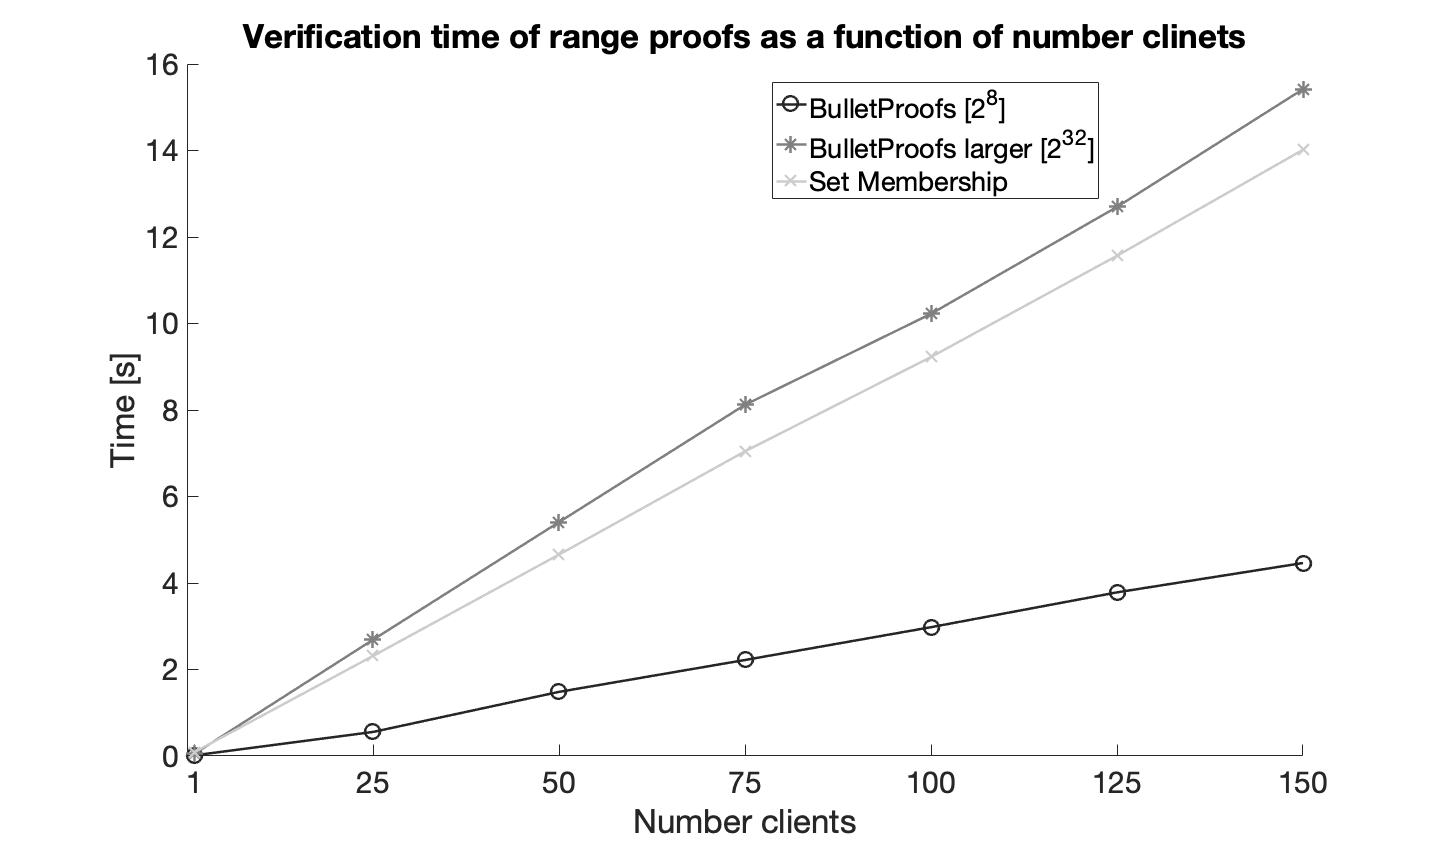
\includegraphics[width=\linewidth]{./figure/verification_nrClients.png}
%\end{figure}

\begin{table}
\caption{Timing in seconds for server and client verifiable-AHSS. Verification of clients is done using three different constructions namely  by implementing  Bulletproofs, signature based range proofs and set membership proofs}
\centering
\label{tab:BenchBP}
\begin{tabular}{l  c c c}

&   \multicolumn{3}{c}{\textbf{Time}}   		\\ 
    																	& Bulletproofs  & Set membership & Aggregated Set membership \\	\toprule
  GenerateShares 				  					&   95/x [$\mu$s]			 &98[$\mu$s]  &98 [$\mu$s]												\\ 
  GenerateRangeProof  						&   53/x [ms]				& 	66 [ms]	&66 [ms]			\\ 
  PartialEval  										&   78/x	[$\mu$s]				&71[$\mu$s]	 		&	71	 [$\mu$s]							\\ 
  PartialProof 									&   273/x[$\mu$s]						& 5255 [$\mu$s]			& 5255 [$\mu$s]				\\ 
   Aggregate										&   -				&		-	&		7947 [$\mu$s]					\\ 
  FinalEval  											&   689/x [ns]						&699  [ns]				&			699  [ns]												\\ 
  FinalProof  												&   50/x	[$\mu$s]			&  115 [$\mu$s]	&				115 [$\mu$s]									\\ 
  VerifyProof	(per client)						  							&   2979/x[ms]					& 9288 [ms]&					9288 [ms]							\\ 
  VerifyServers											&   1672/x [$\mu$s]					&		7947 [ms] 	&		7947 [$\mu$s]					\\ 
  \bottomrule
\end{tabular}
\end{table}